\newcommand{\aps}{funkcije apsolutne vrijednosti}
    Funkcija apsolutne vrijdnosti argumentu pridružuje njegovu udaljenost od nule.
    Dakle ako je argument negativan, množimo ga s \(-1\), a ako je pozitivan ga prepišemo.
    \begin{equation*}
        \begin{split}
            f(x) &= \abs{x} \\
            ako\;je\;x \geq 0,\; f(x) &= x \\
            ako\;je\;x < 0,\; f(x) &= -x
        \end{split}
    \end{equation*}
    Napominjem da sam kod nekih svojstva pretpostavio da geldamo apsolutnu vridnost neke druge funkcije ili složenijeg izraza jer takve slučajeve često viđamo.

\subsubsection{Domena i kodomena \aps}
    Domena kvadratne funkcije je \(\mathbb{R}\), a kodomena \(\mathbb{R^{+}}\).

\subsubsection{Graf \aps}
    Graf funkcije apsolune vrijdnosti jedak je grafu funkcije unutar apsolutne vrijednosti za \(x \geq 0\), a simetričan s obzirom na y-os za \(x < 0\).
    \begin{figure}[ht]
        \centering
        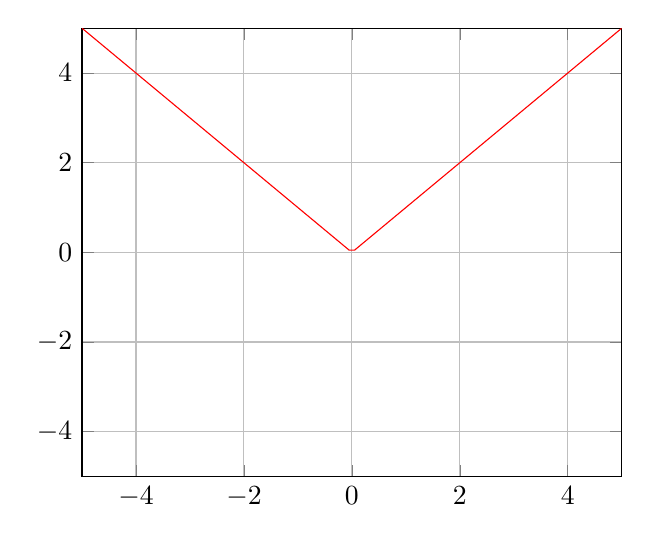
\begin{tikzpicture}
            \begin{axis}[
                grid=major,
                ymin=-5,
                ymax=5,
                xmin=-5,
                xmax=5,
            ]
                \addplot[
                    color = red,
                    samples = 100
                ]{abs(x)};
            \end{axis}
        \end{tikzpicture}
        \caption{Graf funkcije \(f(x) = \abs{x}\)} 
        \label{fig:template}
    \end{figure}

\subsubsection{Nultočke i točke u kojima graf sječe y-os \aps}
    Nultočke i točke u kojima graf sječe y-os određujemo prema definiciji u \ref{nultočke}.
    Ovise o funkciji s kojom je kojom je kvadratna funkcija u kompoziciji.

\subsubsection{Parnost i neparnost \aps}
    Funkcija apsolutne vrijednosti je parna:
    \begin{equation*}
        \begin{split}
            f(x) &= f(-x) \\
            \abs{x} &= \abs{-x}  \\
            x &= x
        \end{split}
    \end{equation*}
    Jednadžba je točna za \(x \geq 0\), ali je analogna za \(x < 0\).
    Funkcija apsolutne vrijdnosti nije neparna jer je parna a nije \(f(x) = 0\).

\subsubsection{Periodičnost \aps}
    Funkcija apsolutne vrijednosti može biti periodnična, no to ovisi o funkciji s kojom je komponirana.
    Na primjer funkcija \(f(x) = \abs{x^2}\) nije periodnična, a funkcija \(f(x) = \abs{sin(x)}\).
    \begin{figure}[ht]
        \centering
        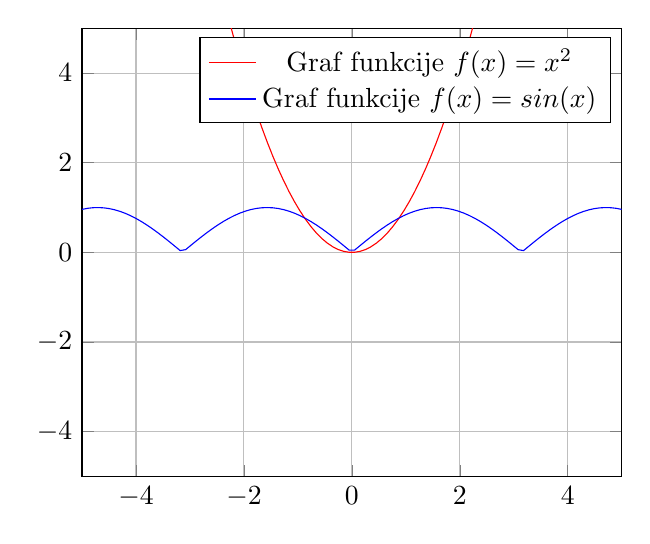
\begin{tikzpicture}
            \begin{axis}[
                grid=major,
                ymin=-5,
                ymax=5,
                xmin=-5,
                xmax=5,
            ]
                \addplot[
                    color = red,
                    samples = 100
                ]{abs(x^2)};
                \addlegendentry{Graf funkcije \(f(x) = \abs{x^2}\)}
                \addplot[
                    color = blue,
                    samples = 100,
                ]{abs(sin(deg(x)))};
                \addlegendentry{Graf funkcije  \(f(x) = \abs{sin(x)}\)}
            \end{axis}
        \end{tikzpicture}
        \caption{Grafovi funkcija apsolunih vrijdnosti komponiranih s periodničnom i neperiodičnom funkcijom}
        \label{fig:template}
    \end{figure}
    \\
\subsubsection{Monotonost \aps}
    Funkcija apsolutne vrijdnosti nije monotona jer je parna.
    Monotona je na intervalima ovisno o funkcija s kojom je u kompoziciji.

\subsubsection{Omeđenost \aps}
    Kvadratna funkcija je po definiciji omeđena odozdo, a donja međa joj je nula.

\subsubsection{Injektivnost i surjektivnost \aps}
    Kvadratna funkcija je surjekcija. Po definiciji iz \ref{injekt}.

\subsubsection{Inverz \aps}
    Kvadratna funkcija nema inverz jer je surjekcija.